
\documentclass[tikz,convert={convertexe={magick.exe}}]{standalone}
\usepackage{tikzsymbols}
\usepackage{MnSymbol,wasysym}

\begin{document}
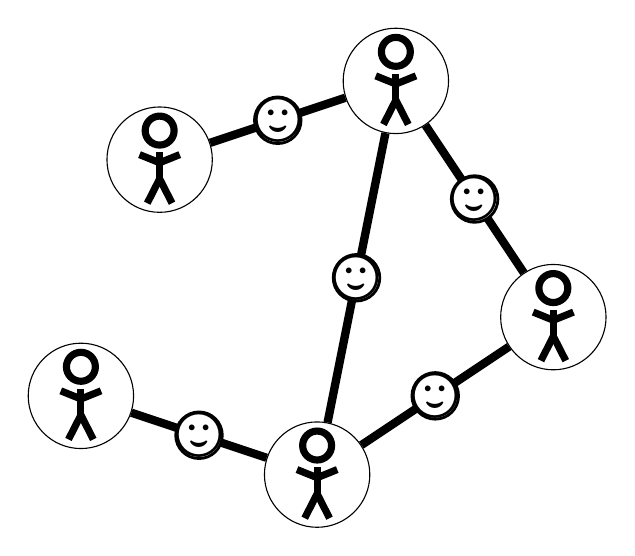
\begin{tikzpicture}[friend/.style={line width=3px}, fn/.style={midway, fill=white, draw, circle, line width=1px, inner sep = -3.2px}]

    
\node (A) at (2,-1) [circle, draw, fill=white, inner sep=0px] {\Strichmaxerl[5]};
\node (B) at (-1,0) [circle, draw, fill=white, inner sep=0px] {\Strichmaxerl[5]};
\node (C) at (3,4) [circle, draw, fill=white, inner sep=0px] {\Strichmaxerl[5]};
\node (D) at (5,1) [circle, draw, fill=white, inner sep=0px] {\Strichmaxerl[5]};
\node (E) at (0,3) [circle, draw, fill=white, inner sep=0px] {\Strichmaxerl[5]};

\draw[friend] (A) -- (B) node[fn]{\Huge\smiley};
\draw[friend] (C) -- (A) node[fn]{\Huge\smiley};
\draw[friend] (D) -- (A) node[fn]{\Huge\smiley};
\draw[friend] (C) -- (D) node[fn]{\Huge\smiley};
\draw[friend] (C) -- (E) node[fn]{\Huge\smiley};

\end{tikzpicture}
\end{document}